\section{Механизмы обеспечения целостности СУБД}

\subsection{Угрозы целостности СУБД}
Задача обеспечения целостности предусматривает комплекс мер по предотвращению непреднамеренного изменения или уничтожения информации, используемой информационной системой управления или системой поддержки принятия решений. Изменение или уничтожение данных может быть следствием неблагоприятного стечения обстоятельств и состояния внешней среды (стихийные бедствия, пожары и т. п.), неадекватных действий пользователей (ошибки при вводе данных, ошибки операторов и т. п.) и проблем, возникающих при многопользовательской обработке данных \autocite{Lihonosov2011}.

Например, с помощью SQL-операторов UPDATE, INSERT и DELETE можно изменить данные в СУБД. Опасность заключается в том, что пользователь, обладающий соответствующими привилегиями, может модифицировать все записи в таблице \autocite{Utebov2008}.

\paragraph{Основные виды и причины возникновения угроз целостности} ~\\

Нарушение целостности информационной базы может произойти по причинам, по которым может произойти и нарушение доступности информации.
Перечислим основные угрозы целостности информации \autocite{Pirogov2009}:

\begin{enumerate}
\item \textbf{Внутренние угрозы целостности ИС}.
    \begin{itemize}
        \item Случайное или умышленное отступление от правил эксплуатации. Например, правила могут предусматривать определенный набор параметров сервера (объем памяти, производительность процессора, объем дискового пространства, версия операционной системы и т.п.), на котором предполагается использовать ИС;
        \item Выход системы из штатного режима эксплуатации в силу случайных или преднамеренных действий пользователей, администраторов и т.д.;
        \item Ошибки конфигурирования системы. В сложных системах конфигурирование выполняется при установке и настройке системы;
        \item Отказ программного обеспечения. Программное обеспечение может содержать ошибки, в том числе и такие, которые могут привести к серьезным повреждениям данных. Кроме этого преднамеренно может быть изменен алгоритм программы. Таким образом, следует защищать программное обеспечение информационной системы и от случайного повреждения, и от исправления непосредственно исполняемых модулей.
    \end{itemize}

\item \textbf{Внешние угрозы целостности ИС}.
    \begin{itemize}
        \item Нарушение условий работы ИС (проблемы с системами связи, отключения электропитания, отопления и т.п.).
        \item Разрушение или повреждение помещений, связанное с природными катаклизмами. Конечно, такая ситуация на первый взгляд кажется мало возможной, но это вполне вероятно в регионах, например, с сейсмической неустойчивостью.
        \item Разрушение информации намеренными действиями человека (диверсия). В данном случае речь идет о действиях людей, не являющихся обслуживающим персоналом данной системы.
        \item Сетевые атаки, вирусные программы и другое вредоносное программное обеспечение.
    \end{itemize}
\end{enumerate}

\paragraph{Способы противодействия} ~\\

Основными средствами защиты целостности информации в ИС являются \autocite{Pirogov2009}:
\begin{itemize}
    \item Транзакционные механизмы, позволяющие восстановить целостность данных в случае незначительных сбоев;
    \item Контроль ввода данных. Много ошибок можно было бы избежать, если программы не пропускали бы заведомо противоречивые данные;
    \item Использование средств защиты целостности СУБД;
    \item Резервное копирование данных;
    \item Периодическое тестирование системы на предмет нарушения целостности.
\end{itemize}

\subsection{Метаданные и словарь данных}

\begin{grayquote}
	\textbf{Метаданные} -- Это данные, описывающие другие данные. Это важный
элемент хранилища данных, который предоставляет возможность показывать пользователю предметно-ориентированную структуру, а не набор абстрактно-связанных таблиц. Метаданные предназначены для хранения
информации о происхождении данных, о любых изменениях данных, о
расположении данных, об ограничениях на данные, о соответствии данных тем или иным объектам предметной области и т. д. \autocite{Pirogov2009}
\end{grayquote}

\paragraph{Назначение словаря данных} ~\\

Согласно канонам реляционной модели данных описание структуры базы
данных (описание объектов, входящих в базу данных) также должно храниться в таблицах. Такая структура называется словарем данных или системным каталогом. По сути, такие данные следует назвать метаданными, т. е. данными, описывающими структуру других
данных.
В 1992 году в стандарте языка SQL было дано описание такого системного
каталога. Но к этому времени в различных СУБД были приняты свои принципы хранения метаданных, отказаться от которых не так-то просто. В результате в одних СУБД вообще отсутствуют стандартные подходы к хранению метаданных, в других эти подходы в значительной степени дополнены своими особенностями. \autocite{Pirogov2009}

\paragraph{Типы словарей данных} ~\\

Существует два типа словарей данных. Активные и пассивные, они отличаются уровнем автоматической синхронизации.

\textbf{Активные словари данных.} Это словари данных, созданные в описываемых ими базах данных, которые автоматически отражают любые изменения внутри этих баз, что позволяет избежать любых несоответствий между словарями данных и описываемыми данными.
\textbf{Словари пассивных данных.} Это словари данных, созданные как отдельные от описываемых ими баз данных сущности. Пассивные словари данных требуют дополнительной логики для синхронизации с базами данных, которые они описывают, и с ними нужно обращаться осторожно.
Компоненты словаря данных
Конкретное содержимое словаря данных может варьироваться. Как правило, эти компоненты представляют собой различные типы метаданных, предоставляющие информацию о данных. \autocite{DataDictionary}

\paragraph{Доступ к словарю данных} ~\\

По 4 правилу Кодда (Dynamic On-Line Catalog Based on the Relational Model) словарь данных должен сохраняться в форме реляционных
таблиц, и СУБД должна поддерживать доступ к нему при
помощи стандартных языковых средств.

Для доступа к словарю данных используются инструкции SQL. Так как словарь данных доступен только для чтения, допускается выполнять только запросы таблиц и представлений.
Можно запрашивать представления словаря, которые основаны на таблицах словаря, чтобы найти сведения, такие как \autocite{Oracle}:
\begin{itemize}
\item определения всех объектов схемы в словаре (таблицы, представления, индексы, синонимы, последовательности, процедуры, функции, пакеты, триггеры и так далее);
\item значения по умолчанию для столбцов;
\item сведения об ограничениях целостности;
\item имена пользователей Oracle;
\item привилегии и роли, предоставленные каждому пользователю;
\item другие общие сведения о базе данных.
\end{itemize}

\paragraph{Состав словаря} ~\\

В состав словаря данных базы данных могут входить: \autocite{DataDictionary}
\begin{itemize}
\item списки объектов данных (имена и определения);
\item свойства элемента данных (такие как тип данных, уникальные идентификаторы, размер, допустимость значений NULL, индексы и параметр required);
\item ER-диаграммы\footnote{Схема «сущность-связь» (также ERD или ER-диаграмма) — это разновидность блок-схемы, где показано, как разные «сущности» (люди, объекты, концепции и так далее) связаны между собой внутри системы.};
\item диаграммы системного уровня;
\item справочные данные — доступные пользователю представления, которые
суммируют и отображают в удобном формате информацию из базовых таблиц словаря. Эти представления декодируют информацию базовых таблиц, представляя ее в полезном виде, таком как имена пользователей или таблиц, чтобы добиться человекочитаемости данных. Большинство пользователей имеют доступ к этим представлениям вместо диаграмм системного уровня;
\item бизнес-логика (например, для проверки качества данных и объектов схемы);
\end{itemize}

Словарь данных базы данных Oracle имеет два основных применения \autocite{Kirillov2009}:
\begin{itemize}
\item Oracle обращается к словарю данных каждый раз, когда выдается предложение DDL;
\item каждый пользователь Oracle может использовать словарь данных как
только читаемый справочник по базе данных.
\end{itemize}

При этом словарь данных всегда доступен при открытой базе данных. Он размещается
в табличном пространстве SYSTEM, которое всегда находится в состоянии online,
когда база данных открыта.

В MongoDB подобными методами получения информации о БД или таблицах являются dbStats, collStatsm rolesInfo и тому подобные.\autocite{MongoDocsCommands}

\paragraph{Представления словаря} ~\\

Рассматривается СУБД от вышеупомянутого Oracle. Словарь данных состоит из нескольких наборов представлений. Во многих случаях такой набор состоит из трех представлений, содержащих аналогичную информацию и отличающихся друг от друга своими префиксами \autocite{Kirillov2009}:
\begin{itemize}
\item USER — представление для пользователя;
\item ALL — расширенное представление для пользователя;
\item DBA — представление администратора.
\end{itemize}

Столбцы в каждом представлении набора идентичны, но имеются исключения. В представлениях с префиксом USER обычно нет столбца с именем OWNER
(владелец); в представлениях USER под владельцем подразумевается пользователь, выдавший запрос. Некоторые представления DBA имеют дополнительные столбцы, которые содержат информацию, полезную для АБД. ~\\

\textbf{Представления с префиксом USER}:
\begin{itemize}
\item отражают окружение пользователя в базе данных, включая информацию
о созданных им объектах, предоставленных им грантах и т. д.;
\item выдают только строки, имеющие отношение к пользователю;
\item имеют столбцы, идентичные с другими представлениями, с тем исключением, что столбец OWNER подразумевается (текущий пользователь);
\item возвращают подмножество информации, предоставляемой представлениями ALL;
\item могут иметь сокращенные общие синонимы для удобства.
\end{itemize}

\textbf{Представления с префиксом ALL} отражают общее представление о базе
данных со стороны пользователя. Эти представления возвращают информацию об объектах, к которым пользователь имеет доступ через общие или явные гранты, помимо тех объектов, которыми владеет этот пользователь. ~\\

\textbf{Представления с префиксом DBA} показывают общее представление о базе
данных, и предназначены для администраторов базы данных.
Во время своей работы Oracle поддерживает набор "виртуальных" таблиц,
в которых регистрируется текущая информация о базе данных. Эти таблицы
называются динамическими таблицами производительности. Так как динамические таблицы производительности не являются истинными таблицами,
большинство пользователей не должно обращаться к ним. Динамические
таблицы производительности принадлежат схеме SYS, а их имена начинаются
с V\_\$. По этим таблицам создаются представления, а для представлений создаются синонимы, имена которых начинаются с V\$.

\subsection{Понятие транзакции}
\begin{grayquote}
Последовательность действий над данными, обрабатываемая СУБД как единая
операция, будем называть \textbf{транзакцией}.
\end{grayquote}
Из определения ясно, что транзакция может состоять из одной или нескольких команд языка SQL. При этом команды языка SQL могут перемежаться
командами, не выполняющими непосредственно операций над данными (не
читающими данные, не изменяющими данные, не изменяющими структуру
данных). Таким образом, в качестве транзакции может быть выбрана любая
часть программы, содержащая команды чтения или записи данных. В частности, транзакция может состоять всего из одной команды, например INSERT,
или из сотен команд, изменяющих или не изменяющих данные.
Понятие транзакции чрезвычайно емкое. Оно в действительности тесно связано с концептуальной моделью данных и всей информационной системы.
Дело в том, что на уровне пользователя операции над данными носят предметный характер: начислить зарплату, уволить работника, перевести деньги
на другой счет и т. п. Для выполнения таких операций часто необходимо выполнить десятки, и даже сотни команд языка SQL. Однако вся эта последовательность команд должна быть подчинена одной цели: операция уровня
пользователя должна быть обязательно выполнена. Что будет, если при выполнении такой цепочки команд произойдет сбой? Как рассматривать тогда
выполняемую операцию — как частично выполненную? Но как в дальнейшем система узнает, что операция была только частично выполнена, и как ее
закончить? Все эти вопросы, в конце концов, и приводят к понятию \textbf{"транзакция"} \autocite{Pirogov2009}.

\paragraph{Фиксация транзакции} ~\\
Согласно требованиям ACID (atomic, consistent, isolated, durable) транзакция должна быть устойчивой. После своего завершения она сохраняется в системе, которую ничто не может вернуть в исходное (до начала транзакции) состояние, т. е. происходит фиксация транзакции, означающая, что ее действие постоянно даже при сбое системы. При выполнении отдельных операций транзакции могут быть нарушены какие-либо требования целостности данных (в первую очередь имеются в виду корпоративные правила целостности, см. главу 2). Однако по окончании выполнения транзакции (фиксация транзакции) все правила целостности базы данных будут соблюдены.
Согласно стандарту транзакция начинается с первой команды, которая обращается к данным. После этого транзакция продолжается до тех пор, пока не будет выполнена команда COMMIT WORK (или просто COMMIT) либо не будет закрыто соединение к базе данных. При выполнении команды COMMIT WORK происходит фиксация транзакции, другими словами, после этой команды откат транзакции уже будет невозможен \autocite{Pirogov2009}.

\paragraph{Прокрутки вперед и назад} ~\\
В результате сбоя СУБД могут возникнуть две потенциальные ситуации \autocite{Karpova2009}:
\begin{itemize}
\item Блоки, содержащие подтверждённые модификации, не были записаны в
файлы данных, так что эти изменения отражены лишь в журнале транзакций. Следовательно, журнал транзакций содержит подтверждённые
данные, которые должны быть переписаны в файлы данных.
\item Журнал транзакций и блоки данных содержат изменения, которые не
были подтверждены. Изменения, внесенные неподтверждёнными
транзакциями, во время восстановления БД должны быть удалены из
файлов данных.
\end{itemize}
Для того чтобы разрешить эти ситуации, СУБД автоматически выполняет два
этапа при восстановлении после сбоев: прокрутку вперед и прокрутку назад.
\begin{enumerate}
 \item Прокрутка вперед заключается в применении к файлам данных всех
изме-нений, зарегистрированных в журнале транзакций. После прокрутки
вперед файлы данных содержат все как подтверждённые, так и
неподтверждённые изменения, которые были зарегистрированы в
журнале транзакций.
 \item Прокрутка назад заключается в отмене всех изменений, которые не были
подтверждены. Для этого используются журнал транзакций и сегменты
отката, информация из которых позволяет определить и отменить те
транзакции, которые не были подтверждены, хотя и попали на диск в
файлы БД.
\end{enumerate}
После выполнения этих этапов восстановления БД находится в согласованном
состоянии и с ней можно работать.

\paragraph{Контрольная точка} ~\\
Критическим моментом в отказе системы является потеря содержимого основной
(оперативной) памяти (в частности, буферов базы данных). Поскольку точное состояние
любой выполнявшейся в момент отказа системы транзакции остается неизвестным, такая транзакция не может быть успешно завершена. Поэтому при перезапуске системы
любая такая транзакция будет отменена (т.е. будет выполнен ее откат).
Более того, при перезапуске системы, возможно, потребуется повторно выполнить некоторые транзакции, которые были успешно завершены
до аварийного останова, но выполненные ими обновления еще не были перенесены из
буферов оперативной памяти в физическую базу данных во вторичной памяти.
Возникает очевидный вопрос: как система определяет в процессе перезапуска, какую
транзакцию следует отменить, а какую выполнить повторно? Ответ заключается в том,
что система автоматически создает контрольные точки с некоторым наперед заданным
интервалом (обычно, когда в журнале накапливается определенное число записей). Для
создания контрольной точки требуется, во-первых, выполнить принудительное сохранение содержимого буферов оперативной памяти в физической базе данных, и, во-вторых,
осуществить принудительное сохранение специальной записи контрольной точки в журнале на физическом носителе. Запись контрольной точки содержит список всех транзакций, выполняемых в тот момент, когда создавалась контрольная точка \autocite{Date2005}.

\paragraph{Откат} ~\\
Для управления транзакциями в системах, поддерживающих механизм
транзакций и язык SQL, используется оператор отката транзакции (отмены изменений): ROLLBACK [WORK]. Для фиксации или отката транзакции
система создаёт неявные точки фиксации и отката.
По команде rollback система откатит транзакцию на начало (на неявную точку
отката).
Для обеспечения целостности транзакции СУБД может откладывать запись
изменений в БД до момента успешного выполнения всех операций, входящих в
транзакцию, и получения команды подтверждения транзакции (commit). Но
чаще используется другой подход: система записывает изменения в БД, не
дожидаясь завершения транзакции, а старые значения данных сохраняет на
время выполнения транзакции в сегментах отката.
Сегмент отката (rollback segment, RBS) – это специальная область памяти на
диске, в которую записывается информация обо всех текущих (незавершённых)
изменениях. Обычно записывается "старое" и "новое" содержимое изменённых
записей, чтобы можно было восстановить прежнее состояние БД при откате
транзакции (по команде rollback) или при откате текущей операции (в случае
возникновения ошибки). Данные в RBS хранятся до тех пор, пока транзакция,
изменяющая эти данные, не будет завершена. Потом они могут быть
перезаписаны данными более поздних транзакций.
Команда savepoint запоминает промежуточную "текущую копию" состояния
базы данных для того, чтобы при необходимости можно было вернуться к
состоянию БД в точке сохранения: откатить работу от текущего момента до
точки сохранения (rollback to <имя\_точки>) или зафиксировать работу от начала
транзакции до точки сохранения (commit to <имя\_точки>). На одну транзакцию
может быть несколько точек сохранения (ограничение на их количество зависит
от СУБД).
Для сохранения сведений о транзакциях СУБД ведёт журнал
транзакций. Журнал транзакций –- это часть БД, в которую поступают данные
обо всех изменениях всех объектов БД. Журнал недоступен пользователям
СУБД и поддерживается особо тщательно (иногда ведутся две копии журнала,
хранимые на разных физических носителях). Форма записи в журнал изменений
зависит от СУБД. Но обычно там фиксируется следующее:
\begin{itemize}
\item номер транзакции (номера присваиваются автоматически по возрастанию);
\item состояние транзакции (завершена фиксацией или откатом, не завершена,
находится в состоянии ожидания);
\item точки сохранения (явные и неявные);
\item команды, составляющие транзакцию, и проч.
\end{itemize}
Начало транзакции соответствует появлению первого исполняемого SQLоператора. При этом в журнале появляется запись об этой транзакции \autocite{Karpova2009}.

\paragraph{Транзакции как средство изолированности пользователей} ~\\

Поддержание механизма транзакций —- показатель уровня развитости СУБД
и основа обеспечения целостности базы данных. Транзакции также составляют основу изолированности в многопользовательских системах, где с одной базой данных параллельно могут работать несколько пользователей
и (или) прикладных программ. Одна из основных задач СУБД —- обеспечение изолированности, т. е. создание такого режима функционирования, при
котором каждому пользователю казалось бы, что база данных доступна только ему. Такую задачу СУБД принято называть параллелизмом транзакций.
Большинство выполняемых действий производится в теле транзакций. По
умолчанию каждая команда выполняется как самостоятельная транзакция.
Как было показано ранее, при необходимости пользователь может явно указать ее начало и конец, чтобы иметь возможность включить в нее несколько
команд.
Решение проблемы параллельной обработки базы данных заключается в том,
что строки таблиц блокируются, а последующие транзакции, модифицирующие эти строки, отвергаются и переводятся в режим ожидания. В связи со
свойством сохранения целостности базы данных транзакции являются подходящими единицами изолированности пользователей. Действительно, если каждый сеанс взаимодействия с базой данных реализуется транзакцией, то
пользователь начинает с того, что обращается к согласованному состоянию
базы данных — состоянию, в котором она могла бы находиться, даже если
бы пользователь работал с ней в одиночку.
Если бы в СУБД не были реализованы механизмы блокирования, то при
одновременном чтении и изменении одних и тех же данных несколькими
пользователями могли бы возникнуть проблемы одновременного доступа.


\paragraph{Конфликты транзакций и уровни изоляции} ~\\

Уровни изоляции определяют степень, в которой транзакция должна быть изолирована от изменений данных, сделанных любой другой транзакцией в системе базы данных. Уровни изоляции отличаются разрешениями следующих конфликтов:
\begin{itemize}
\item \textbf{Потерянное обновление (lost update)} — когда несколько транзакций что-то обновили в БД, но по итогам результат такой, будто отработала лишь часть транзакций. Самый опасный побочный эффект, по сути, полное отсутствие изоляции транзакций — две транзакции читают одну ячейку, записывают изменённое значение (одна вычитает стоимость мороженого, другая плату за квартиру). В итоге в ячейке значение от второй транзакции, а первой как будто и не было.
\item \textbf{Грязное чтение (dirty read)} — ситуация, когда транзакция считывает данные, которые еще не были зафиксированы. Например, транзакция 1 обновляет строку и оставляет ее незафиксированной, в то время как транзакция 2 читает обновленную строку. Если транзакция 1 откатывает изменение, транзакция 2 будет считывать данные, которые считаются никогда не существовавшими.
\item \textbf{Неповторяемое чтение (non-repeatable read)} — когда транзакция дважды считывает одну и ту же строку и каждый раз получает другое значение. Например, предположим, что транзакция T1 считывает данные. Из-за параллелизма другая транзакция T2 обновляет те же данные и фиксирует их. Теперь, если транзакция T1 повторно считывает те же данные, она получит другое значение.
\item \textbf{Фантомное чтение (phantom reads)} — когда выполняются два одинаковых запроса, но извлекаемые ими строки различаются. Например, транзакция T1 извлекает набор строк, удовлетворяющих некоторым критериям поиска. Далее транзакция T2 создает несколько новых строк, соответствующих критериям поиска для транзакции T1. Если транзакция T1 повторно выполняет инструкцию, которая считывает строки, на этот раз она получает другой набор строк. Отличие от предыдущего пункта в том, что в этом случае происходит агрегация строк, а в предыдущем происходит чтение лишь одной строки.
\end{itemize}

Основываясь на политиках разрешения перечисленных конфликтов, стандарт SQL определяет четыре уровня изоляции:
\begin{itemize}
\item \textbf{Read Uncommitted} — это самый низкий уровень изоляции. На этом уровне одна транзакция может считывать еще не зафиксированные изменения, сделанные другими транзакциями, тем самым допуская грязное чтение. На этом уровне транзакции не изолированы друг от друга.
\item \textbf{Read Committed} — уровень изоляции гарантирует, что любые считанные данные фиксируются в момент их чтения. Таким образом, он не допускает грязного чтения. Транзакция удерживает блокировку чтения или записи для текущей строки и, таким образом, предотвращает ее чтение, обновление или удаление другими транзакциями.
\item \textbf{Repeatable Read} — транзакция удерживает блокировки чтения для всех строк, на которые она ссылается, и записывает блокировки для указанных строк для действий обновления и удаления. Поскольку другие транзакции не могут читать, обновлять или удалять эти строки, следовательно, это позволяет избежать неповторяющегося чтения.
\item \textbf{Serializable} — самый высокий уровень изоляции. Выполнение определяется как выполнение операций, в которых одновременно выполняемые транзакции кажутся последовательно выполняемыми\autocite{BeginningSQL}.
\end{itemize}

\begin{table}
\begin{tabular}{l|l|l|l|l}
                 & Фантомное чтение         & Неповторяющееся чтение   & Грязное чтение           & Потерянное обновление    \\ \hline
Serializable     & \cellcolor[HTML]{32CB00} & \cellcolor[HTML]{32CB00} & \cellcolor[HTML]{32CB00} & \cellcolor[HTML]{32CB00} \\ \hline
Repeatable Read  & \cellcolor[HTML]{FE0000} & \cellcolor[HTML]{32CB00} & \cellcolor[HTML]{32CB00} & \cellcolor[HTML]{32CB00} \\ \hline
Read Committed   & \cellcolor[HTML]{FE0000} & \cellcolor[HTML]{FE0000} & \cellcolor[HTML]{32CB00} & \cellcolor[HTML]{32CB00} \\ \hline
Read Uncommitted & \cellcolor[HTML]{FE0000} & \cellcolor[HTML]{FE0000} & \cellcolor[HTML]{FE0000} & \cellcolor[HTML]{32CB00} \\ \hline
\end{tabular}
\end{table}


\paragraph{Методы сериализации транзакций} ~\\

Делятся на три типа:
\begin{itemize}
\item \textbf{С блокирующим планировщиком (blocking sheduller)} — для каждого запроса планировщик запрашивает блокировку. Каждая блокировка запрашивается в определенном режиме (чтение или запись). Если запрашиваемый элемент данных еще не заблокирован в несовместимом режиме, блокировка предоставляется; в противном случае возникает конфликт блокировок и транзакция блокируется, пока текущий владелец блокировки не освободит блокировку. Например: двухфазные AL (Altruistic Locking), O2PL (Ordered Sharing of Locks), 2PL (Two-Phase Locking), C2PL (Conservative Two-Phase Locking), S2PL (Strict Two-Phase Locking), SS2PL (Strong Strict Two-Phase Locking), не двухфазные WTL (Write-only Tree Locking), RWTL (Read-Write Tree Locking).

\item \textbf{С неблокирующим планировщиком (non-blocking sheduller)} — запрос отрабатывает, не имея возможности заблокировать другой запрос, конфликты разрешаются постфактум. Например: TO (Timestamp Ordering), SGT (Serialization Graph Testing).

\item \textbf{Смешанный} — использует разные типы для разных видов конфликтов (rw/wr, ww).\autocite{TransactionalInformationSystems}
\end{itemize}

\subsection{Блокировки} ~\\

Блокировки, называемые также синхронизационными захватами объектов, могут быть применены к разному типу объектов. Наибольшим объектом блокировки может быть вся БД, однако этот вид блокировки сделает БД недоступной для всех приложений, которые работают с данной БД. Следующий тип объекта блокировки —- это таблицы. Транзакция, которая работает с таблицей, блокирует ее на все время выполнения транзакции. Этот вид блокировки предпочтительнее предыдущего, потому что позволяет параллельно выполнять транзакции, которые работают с другими таблицами.

В ряде СУБД реализована блокировка на уровне страниц. В этом случае СУБД блокирует только отдельные страницы на диске, когда транзакция обращается к ним. Этот вид блокировки еще более мягок и позволяет разным транзакциям работать даже с одной и той же таблицей, если они обращаются к разным страницам данных.

В некоторых СУБД возможна блокировка на уровне строк, однако такой механизм блокировки требует дополнительных затрат на поддержку этого вида блокировки.

В настоящее время проблема блокировок является предметом большого числа исследований \autocite{Intuit}.

\paragraph{Режимы блокировок} ~\\

Рассматривают два типа блокировок (синхронизационных захватов) \autocite{Intuit}:
\begin{itemize}
\item совместный режим блокировки — нежесткая, или разделяемая, блокировка, обозначаемая как S (Shared). Этот режим обозначает разделяемый захват объекта и требуется для выполнения операции чтения объекта. Объекты, заблокированные таким образом, не изменяются в ходе выполнения транзакции и доступны другим транзакциям также, но только в режиме чтения;
\item монопольный режим блокировки — жесткая, или эксклюзивная, блокировка, обозначаемая как X (eXclusive). Данный режим блокировки предполагает монопольный захват объекта и требуется для выполнения операций занесения, удаления и модификации. Объекты, заблокированные данным типом блокировки, фактически остаются в монопольном режиме обработки и недоступны для других транзакций до момента окончания работы данной транзакции.
\end{itemize}
\paragraph{Правила согласования блокировок}~\\

Захваты объектов несколькими транзакциями по чтению совместимы, то есть нескольким транзакциям допускается читать один и тот же объект, захват объекта одной транзакцией по чтению не совместим с захватом другой транзакцией того же объекта по записи, и захваты одного объекта разными транзакциями по записи не совместимы. В примере, представленном на рис. 1 считается, что первой блокирует объект транзакция А, а потом пытается получить к нему доступ транзакция В.

\begin{figure}[h!]
    \centering
    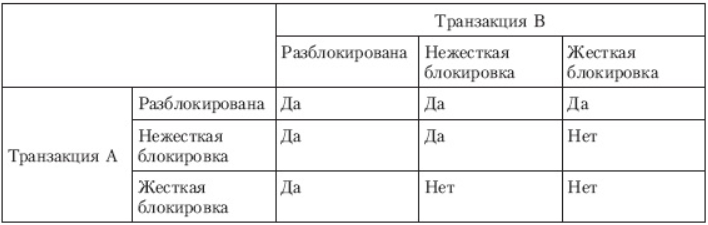
\includegraphics[width=0.8\textwidth]{assets/blocks.PNG}
    \caption{Правила применения жесткой и нежесткой блокировок транзакций}
\end{figure}


\paragraph{Двухфазный протокол синхронизационных блокировок}~\\

В базах данных и обработке транзакций двухфазная блокировка (2PL) — это метод управления параллелизмом, который гарантирует сериализуемость. Так же называют результирующий набор графиков транзакций базы данных (истории). Протокол использует блокировки, применяемые транзакцией к данным, которые могут блокировать (интерпретировать как сигналы для остановки) другие транзакции от доступа к тем же данным в течение жизни транзакции.

По протоколу 2PL блокировки (locks) применяются и удаляются в два этапа:
\begin{enumerate}
\item Фаза расширения: блокировки берутся и ни одна блокировка не освобождается.
\item Фаза сокращения: блокировки освобождаются и ни одна блокировка не берётся.
\end{enumerate}

В базовом протоколе используются два типа блокировок: Shared и Exclusive locks. Уточнения базового протокола могут использовать больше типов блокировок. Используя блокировки, блокирующие процессы, 2PL могут подвергаться взаимоблокировкам, которые являются результатом взаимной блокировки двух или более транзакций \autocite{Wiki}.

\paragraph{Тупиковые ситуации, их распознавание и разрушение} ~\\

Одним из наиболее чувствительных недостатков метода сериализации транзакций на основе синхронизационных захватов является возможность возникновение тупиков (deadlocks) между транзакциями.

Вот простой пример возникновения тупика между транзакциями T1 и T2:
\begin{enumerate}
\item транзакции T1 и T2 установили монопольные захваты объектов r1 и r2 соответственно;
\item после этого T1 требуется совместный захват r2, а T2 - совместный захват r1;
\item ни одна из транзакций не может продолжаться, следовательно, монопольные захваты не будут сняты, а совместные - не будут удовлетворены.
\end{enumerate}
Поскольку тупики возможны, и никакого естественного выхода из тупиковой ситуации не существует, то эти ситуации необходимо обнаруживать и искусственно устранять.

Основой обнаружения тупиковых ситуаций является построение (или постоянное поддержание) графа ожидания транзакций. Граф ожидания транзакций - это ориентированный двудольный граф, в котором существует два типа вершин - вершины, соответствующие транзакциям, и вершины, соответствующие объектам захвата. В этом графе существует дуга, ведущая из вершины-транзакции к вершине-объекту, если для этой транзакции существует удовлетворенный захват объекта. В графе существует дуга из вершины-объекта к вершине-транзакции, если транзакция ожидает удовлетворения захвата объекта.

Легко показать, что в системе существует ситуация тупика, если в графе ожидания транзакций имеется хотя бы один цикл.

Для распознавание тупика периодически производится построение графа ожидания транзакций (как уже отмечалось, иногда граф ожидания поддерживается постоянно), и в этом графе ищутся циклы. Традиционной техникой (для которой существует множество разновидностей) нахождения циклов в ориентированном графе является редукция графа.

Не вдаваясь в детали, редукция состоит в том, что прежде всего из графа ожидания удаляются все дуги, исходящие из вершин-транзакций, в которые не входят дуги из вершин-объектов. (Это как бы соответствует той ситуации, что транзакции, не ожидающие удовлетворения захватов, успешно завершились и освободили захваты). Для тех вершин-объектов, для которых не осталось входящих дуг, но существуют исходящие, ориентация исходящих дуг изменяется на противоположную (это моделирует удовлетворение захватов). После этого снова срабатывает первый шаг и так до тех пор, пока на первом шаге не прекратится удаление дуг. Если в графе остались дуги, то они обязательно образуют цикл.

Предположим, что нам удалось найти цикл в графе ожидания транзакций. Что делать теперь? Нужно каким-то образом обеспечить возможность продолжения работы хотя бы для части транзакций, попавших в тупик. Разрушение тупика начинается с выбора в цикле транзакций так называемой транзакции-жертвы, т.е. транзакции, которой решено пожертвовать, чтобы обеспечить возможность продолжения работы других транзакций.

Грубо говоря, критерием выбора является стоимость транзакции; жертвой выбирается самая дешевая транзакция. Стоимость транзакции определяется на основе многофакторная оценка, в которую с разными весами входят время выполнения, число накопленных захватов, приоритет.

После выбора транзакции-жертвы выполняется откат этой транзакции, который может носить полный или частичный характер. При этом, естественно, освобождаются захваты и может быть продолжено выполнение других транзакций.

Естественно, такое насильственное устранение тупиковых ситуаций является нарушением принципа изолированности пользователей, которого невозможно избежать.

Заметим, что в централизованных системах стоимость построения графа ожидания сравнительно невелика, но она становится слишком большой в по-настоящему распределенных СУБД, в которых транзакции могут выполняться в разных узлах сети. Поэтому в таких системах обычно используются другие методы сериализации транзакций.

Еще одно замечание. Чтобы минимизировать число конфликтов между транзакциями, в некоторых СУБД (например, в Oracle) используется следующее развитие подхода. Монопольный захват объекта блокирует только изменяющие транзакции. После выполнении операции модификации предыдущая версия объекта остается доступной для чтения в других транзакциях. Кратковременная блокировка чтения требуется только на период фиксации изменяющей транзакции, когда обновленные объекты становятся текущими \autocite{Serial}
\subsection{Ссылочная целостность}
Ссылочная целостность. Ссылочная целостность относится непосредственно к связям между таблицами. Если кратко, то ссылочная целостность
должна отвечать на вопрос: что будет со строками одной таблицы, если в
связанной таблице выполняется какая-либо операция модификации? Для
того чтобы понять логику ссылочной целостности, будем считать таблицу
главной в паре связанных таблиц, если она содержит первичный ключ, с
помощью которого осуществляется связь. Вторую таблицу будем считать
подчиненной таблицей. Теперь выделим три вида операции над связанными таблицами: удаление из главной таблицы, обновление строк главной
таблицы, вставка в подчиненную таблицу.
\begin{enumerate}
\item Удаление строк из главной таблицы. Если удаляемая строка не связана
со строками другой таблицы, то удалять можно без всяких последствий. Но если удаляемая строка связана со строками другой таблицы, то
надо подумать, что же будет с этими строками. Просто оставить их без
изменения нельзя, т. к. не понятно, как быть со значениями внешних
ключей. В принципе, возможны следующие четыре сценария, поддерживаемые основными СУБД:
\begin{itemize}
\item строки из подчиненной таблицы должны быть удалены вместе со
связанными строками из подчиненной таблицы. Такой механизм называется каскадированием;
\item если удаляемая строка из главной таблицы связана со сроками из
подчиненной таблицы, то такая операция удаления должна быть отвергнута. Данный механизм наиболее безопасен и предпочтителен
при построении информационной системы;
\item если строка в подчиненной таблице связана с удаляемой строкой в
главной таблице, то внешнему ключу следует присвоить значение
NULL;
\item если строка в подчиненной таблице связана с удаляемой строкой в
главной таблице, то внешнему ключу следует присвоить значение,
принятое по умолчанию.
\end{itemize}
\item Обновление строк из главной таблицы. Если обновляемая строка не
связана со строками другой таблицы или обновляются столбцы, не от-
носящиеся к первичному ключу, то обновлять можно без всяких по-
следствий. Но если обновляемая строка связана со строками другой
таблицы и обновляется первичный ключ, то здесь, как и в предыдущем
случае, возможны четыре сценария:
\begin{itemize}
\item первичные ключи из главной таблицы обновляются вместе с внеш-
ними ключами подчиненной таблицы. Как и в случае с подобной
операцией удаления, этот механизм называется каскадированием;
\item если обновляемая строка связана с какой-либо строкой подчиненной
таблицы, то операция обновления должна быть отвергнута;
\item если строка в подчиненной таблице связана с обновляемой строкой в
главной таблице, то внешнему ключу следует присвоить значение
NULL;
\item если строка в подчиненной таблице связана с обновляемой строкой в
главной таблице, то внешнему ключу следует присвоить значение,
принятое по умолчанию.
\end{itemize}
\item Вставка строк в подчиненную таблицу. Здесь возможны следующие
механизмы.
\begin{itemize}
    \item Строка в подчиненной таблице вставляется вместе со строкой в
главной таблице. Здесь важно иметь в виду, что в главной таблице
для всех столбцов должны быть определены значения по умолча-
нию. Последовательность добавления такая: вначале добавляется
строка в главную таблицу и определяется значение первичного клю-
ча. Затем добавляется строка в подчиненную таблицу, в которой
значению внешнего ключа присваивается значение первичного клю-
ча в главной таблице.
\item Строка в подчиненную таблицу добавляется только при условии,
что соответствующая ей строка в главной таблице уже существует.
\item При добавлении строки в подчиненную таблицу внешнему ключу
присваивается значение NULL.
\item При добавлении строки в подчиненную таблицу внешнему ключу
присваивается значение по умолчанию.
\end{itemize}
\end{enumerate}
В некоторых простых СУБД отсутствует возможность устанавливать
связи между таблицами и, таким образом, поддерживать ссылочную целостность. В этом случае поддержание ссылочной целостности полностью ложится на плечи программиста. Другими словами, связь между таблицами должна быть реализована на уровне прикладного программного обеспечения.
\paragraph{Декларативная и процедурная ссылочные целостности} ~\\
Различают два способа реализации ограничений целостности:
\begin{itemize}
\item Декларативная поддержка ограничений целостности.
\item Процедурная поддержка ограничений целостности.
\end{itemize}
\begin{grayquote}
\textbf{Декларативная поддержка ограничений целостности} заключается в определении ограничений средствами языка определения данных (DDL - Data Definition Language). Обычно средства декларативной поддержки целостности (если они имеются в СУБД) определяют ограничения на значения доменов и атрибутов, целостность сущностей (потенциальные ключи отношений) и ссылочную целостность (целостность внешних ключей). Декларативные ограничения целостности можно использовать при создании и модификации таблиц средствами языка DDL или в виде отдельных утверждений (ASSERTION).
\end{grayquote}

Например, следующий оператор создает таблицу PERSON и определяет для нее некоторые ограничения целостности:

\begin{verbatim}
CREATE TABLE PERSON
  (Pers_Id INTEGER PRIMARY KEY,
  Pers_Name CHAR(30) NOT NULL,
  Dept_Id REFERENCES DEPART(Dept_Id) ON UPDATE CASCADE ON DELETE CASCADE);
\end{verbatim}

После выполнения оператора для таблицы PERSON будут объявлены следующие ограничения целостности:
\begin{itemize}
\item Поле Pers\_Id образует потенциальный ключ отношения.
\item Поле Pers\_Name не может содержать null-значений.
\item Поле Dept\_Id является внешней ссылкой на родительскую таблицу DEPART, причем, при изменении или удалении строки в родительской таблице каскадно должны быть внесены соответствующие изменения в дочернюю таблицу.
\end{itemize}
\begin{grayquote}
\textbf{Процедурная поддержка ограничений целостности} заключается в использовании триггеров и хранимых процедур.
\end{grayquote}

Не все ограничения целостности можно реализовать декларативно. Примером такого ограничения может служить требование из примера 1, утверждающее, что поле Dept\_Kol таблицы DEPART должно содержать количество сотрудников, реально числящихся в подразделении. Для реализации этого ограничения необходимо создать триггер, запускающийся при вставке, модификации и удалении записей в таблице PERSON, который корректно изменяет значение поля Dept\_Kol. Например, при вставке в таблицу PERSON новой строки, триггер увеличивает на единицу значение поля Dept\_Kol, а при удалении строки - уменьшает. Заметим, что при модификации записей в таблице PERSON могут потребоваться даже более сложные действия. Действительно, модификация записи в таблице PERSON может заключаться в том, что мы переводим сотрудника из одного отдела в другой, меняя значение в поле Dept\_Id. При этом необходимо в старом подразделении уменьшить количество сотрудников, а в новом - увеличить \autocite{TransCit}.
\paragraph{Внешний ключ} ~\\
\begin{grayquote}
\textbf{Внешний ключ} – это ограничение целостности, в соответствии с которым
множество значений внешнего ключа является подмножеством значений
первичного или уникального ключа родительской таблицы \autocite{Karpova2009}.
\end{grayquote}

Ограничение целостности по внешнему ключу проверяется в двух случаях \autocite{Karpova2009}:
\begin{itemize}
    \item при добавлении записи в подчинённую таблицу СУБД проверяет, что в
родительской таблице есть запись с таким же значением первичного
ключа;
    \item при удалении записи из родительской таблицы СУБД проверяет, что в
подчинённой таблице нет записей с таким же значением внешнего ключа.
\end{itemize}

\paragraph{Способы поддержания ссылочной целостности} ~\\
СУБД имеют механизм автоматического поддержания ссылочной целостности. Любая операция, изменяющая данные в таблице, вызывает автоматическую проверку ссылочной целостности. При этом \autocite{WikiLink}:
\begin{itemize}
    \item При операции добавления записи автоматически проверяется, ссылаются ли внешние ключи в этой записи на существующие записи в заявленных при описании связанных таблицах. Если выясняется, что операция приведёт к появлению некорректных ссылок, она не выполняется — система возвращает ошибку.
    \item При операции редактирования записи проверяется:
    \begin{itemize}
        \item если изменяется её первичный ключ и на данную запись имеются ссылки, то операция редактирования завершается с ошибкой;
        \item если изменяется какой-то из внешних ключей, хранящихся в этой записи, и после изменения внешний ключ будет ссылаться на несуществующую запись, то операция редактирования завершается с ошибкой.
    \end{itemize}
    \item При операции удаления записи проверяется, нет ли на неё ссылок. Если ссылки имеются, то возможно три варианта дальнейших действий (фактически выполняемый зависит от СУБД и от выбора программиста, который он должен сделать при описании связи):
    \begin{itemize}
        \item Запрет — удаление блокируется и возвращается ошибка.
        \item Каскадное удаление — в одной транзакции производится удаление данной записи и всех записей, ссылающихся на данную. Если на удаляемые записи также есть ссылки и настройки также требуют удаления, то каскадное удаление продолжается дальше. Таким образом, после удаления данной записи в базе не остаётся ни одной записи, прямо или косвенно ссылающейся на неё. Если хотя бы одну из ссылающихся записей удалить не получается (либо для неё настроен запрет, либо происходит какая-либо ещё ошибка), то все удаления запрещаются.
        \item Присвоение NULL — во все внешние ключи записей, ссылающихся на данную, записывается маркер NULL. Если хотя бы для одной из ссылающихся записей это невозможно (например, если поле внешнего ключа описано как NOT NULL), то удаление запрещается.
    \end{itemize}
\end{itemize}

\subsection{Правила (триггеры)}
Триггеры являются одной из разновидностей хранимых процедур. Их исполнение происходит при выполнении для таблицы какого-либо оператора языка манипулирования данными (DML). Триггеры используются для проверки целостности данных, а также для отката транзакций.

Триггер представляет собой специальный тип хранимых процедур, запускаемых сервером автоматически при попытке изменения данных в таблицах, с которыми триггеры связаны. Каждый триггер привязывается к конкретной таблице. Все производимые им модификации данных рассматриваются как одна транзакция. В случае обнаружения ошибки или нарушения целостности данных происходит откат этой транзакции. Тем самым внесение изменений запрещается. Отменяются также все изменения, уже сделанные триггером.

Триггер представляет собой весьма полезное и в то же время опасное средство. Так, при неправильной логике его работы можно легко уничтожить целую базу данных, поэтому триггеры необходимо очень тщательно отлаживать.

В отличие от обычной подпрограммы, триггер выполняется неявно в каждом случае возникновения триггерного события, к тому же он не имеет аргументов. Приведение его в действие иногда называют запуском триггера \autocite{IntuitTrigg}

\paragraph{Цели использования правил} ~\\

С помощью триггеров достигаются следующие цели \autocite{IntuitTrigg}:
\begin{itemize}
\item проверка корректности введенных данных и выполнение сложных ограничений целостности данных, которые трудно, если вообще возможно, поддерживать с помощью ограничений целостности, установленных для таблицы;
\item выдача предупреждений, напоминающих о необходимости выполнения некоторых действий при обновлении таблицы, реализованном определенным образом;
\item накопление аудиторской информации посредством фиксации сведений о внесенных изменениях и тех лицах, которые их выполнили;
\item поддержка репликации.
\end{itemize}
\paragraph{Способы задания, моменты выполнения} ~\\

Создает триггер только владелец базы данных. Это ограничение позволяет избежать случайного изменения структуры таблиц, способов связи с ними других объектов и т.п.
Основной формат команды CREATE TRIGGER показан ниже:
\begin{verbatim}
<Определение_триггера>::=
  CREATE TRIGGER имя_триггера
  BEFORE | AFTER <триггерное_событие>
  ON <имя_таблицы>
  [REFERENCING
    <список_старых_или_новых_псевдонимов>]
  [FOR EACH { ROW | STATEMENT}]
  [WHEN(условие_триггера)]
  <тело_триггера>
\end{verbatim}

Триггерные события состоят из вставки, удаления и обновления строк в таблице. В последнем случае для триггерного события можно указать конкретные имена столбцов таблицы.

Триггер – это процедура БД, которая привязана к конкретной таблице и вызывается
автоматически при наступлении определённого события
(добавления, удаления или модификации данных этой таблицы).

В отличие от обычной подпрограммы, триггер выполняется неявно в каждом случае возникновения триггерного события, к тому же он не имеет аргументов. Приведение его в действие иногда называют запуском триггера.

Время запуска триггера определяется с помощью ключевых слов BEFORE ( триггер запускается до выполнения связанных с ним событий) или AFTER (после их выполнения).

Выполняемые триггером действия задаются для каждой строки ( FOR EACH ROW ), охваченной данным событием, или только один раз для каждого события ( FOR EACH STATEMENT ).

Обозначение <список\_старых\_или\_новых\_псевдонимов> относится к таким компонентам, как старая или новая строка ( OLD / NEW ) либо старая или новая таблица ( OLD TABLE / NEW TABLE ). Ясно, что старые значения не применимы для событий вставки, а новые – для событий удаления \autocite{IntuitTrigg}.

\subsection{События}

\paragraph{Назначение механизма событий} ~\\

Механизм событий в базе данных (database events) позволяет прикладным программам и серверу базы данных уведомлять другие программы о наступлении в базе данных определенного события и тем самым синхронизировать их работу \autocite{OSP}.

\paragraph{Сигнализаторы событий. Типы уведомлений о происхождении события. Компоненты механизма событий} ~\\

Операторы языка SQL, обеспечивающие уведомление, часто называют сигнализаторами событий в базе данных (database event alerters). Функции управления событиями целиком ложатся на сервер базы данных.

Механизм событий используется следующим образом. Вначале в базе данных для каждого события создается флажок, состояние которого будет оповещать прикладные программы о том, что некоторое событие имело место (оператор CREATE DBEVENT - СОЗДАТЬ СОБЫТИЕ). Далее во все прикладные программы, на ход выполнения которых может повлиять это событие, включается оператор REGISTER DBEVENT (ЗАРЕГИСТРИРОВАТЬ СОБЫТИЕ), который оповещает сервер базы данных, что данная программа заинтересована в получении сообщения о наступлении события. Теперь любая прикладная программа или процедура базы данных может вызвать событие оператором RAISE DBEVENT (ВЫЗВАТЬ СОБЫТИЕ). Как только событие произошло, каждая зарегистрированная программа может получить его, для чего должна запросить очередное сообщение из очереди событий (оператор GET DBEVENT - ПОЛУЧИТЬ СОБЫТИЕ) и запросить информацию о событии, в частности, его имя (оператор SQL INQUIRE\_SQL) \autocite{OSP}.
